\chapter{Diseño}

En este capítulo se abordarán las cuestiones de diseño la interfaz de usuario, explicando de manera detallada cada elemento que la compone, junto a algunos bocetos. Además, se incluirá un diagrama de navegación para saber a qué pantallas lleva cada opción.

\bigskip

Cada cuestión anteriormente mencionada se dividirá en secciones a continuación:

\section{Diseño de la Interfaz de Usuario}

% rescribir
% El diseño de la interfaz de usuario en el configurador de la simulación está compuesto por dos secciones principales: una primera a la izquierda para configurar el número de vehículos, la disciplina, el número de pilotos y las opciones de importación y exportación de la configuración, y una segunda sección a la derecha consistente en las características que tiene cada piloto, junto al botón de comenzar la simulación.

La interfaz de usuario del configurador de la simulación está dividida en dos secciones principales: a la izquierda se encuentra la sección para el número de vehículos y de pilotos, la disciplina y las opciones de importación y exportación de la configuración. A la derecha está la segunda sección, compuesta por las características de cada piloto y el botón para comenzar la simulación.

\bigskip

% rescribir
% Mientras que durante la carrera, aparecerá un listado de posiciones de los pilotos y un contador de vueltas a la izquierda. El listado permitirá visualizar y modificar el estado de cada piloto en tiempo real. La disposición de los elementos en esta pantalla será muy similar a disciplinas como la Formula 1, cuyo listado de posición y contador de vueltas se encuentran a la izquierda y en cada celda del listado aparecen las 3 primeras iniciales del apellido. En mi caso he decidido también añadir la primera letra del nombre, por si se da el caso de que hay varios pilotos con el mismo apellido.

Durante la carrera, se mostrará un listado de posiciones de los pilotos y un contador de vueltas en la parte izquierda de la pantalla. Este listado permitirá visualizar y modificar el estado de cada piloto en tiempo real. La disposición de los elementos será similar a la de disciplinas como la Fórmula 1, donde el ranking de pilotos y el contador de vueltas aparecen a la izquierda, y en cada celda de posición aparecen las tres primeras letras del apellido. En este proyecto, he decidido añadir también la primera letra del nombre, en caso de que haya varios pilotos con el mismo apellido.

\bigskip

A continuación se encuentran algunos bocetos de ambas pantallas:

\begin{figure}[H]
    \centering
    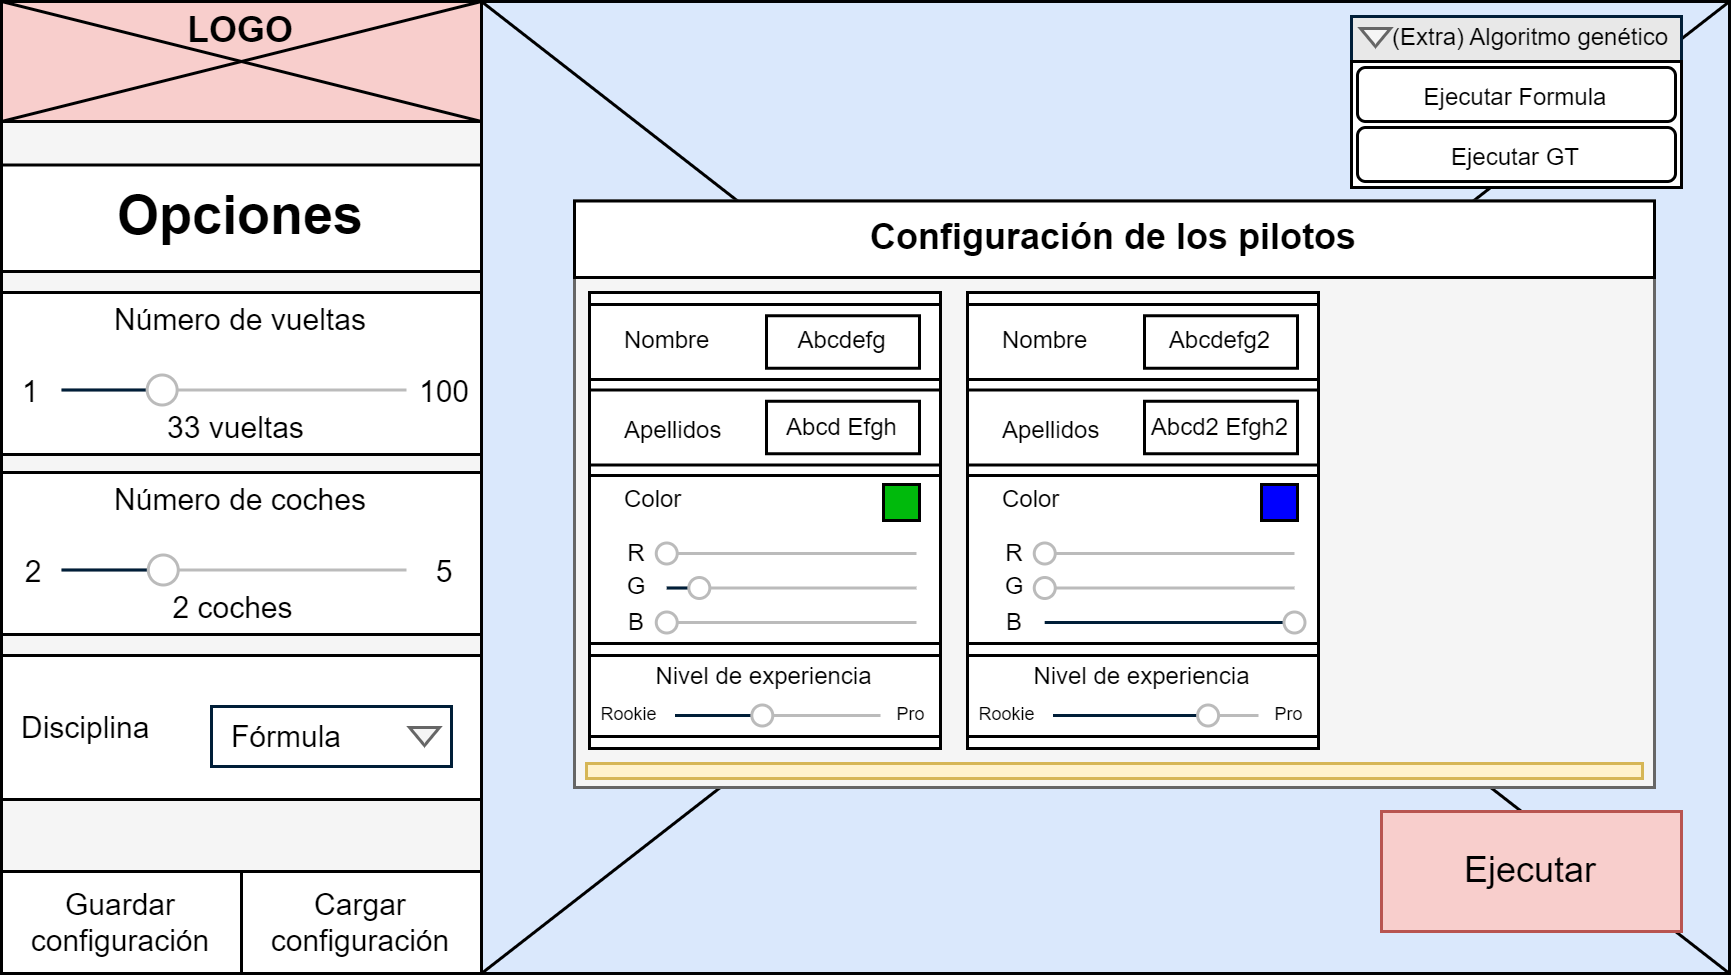
\includegraphics[width=\textwidth]{imagenes/pag1.png}
    \caption{Interfaz del configurador antes de la carrera.}
\end{figure}

\begin{figure}[H]
    \centering
    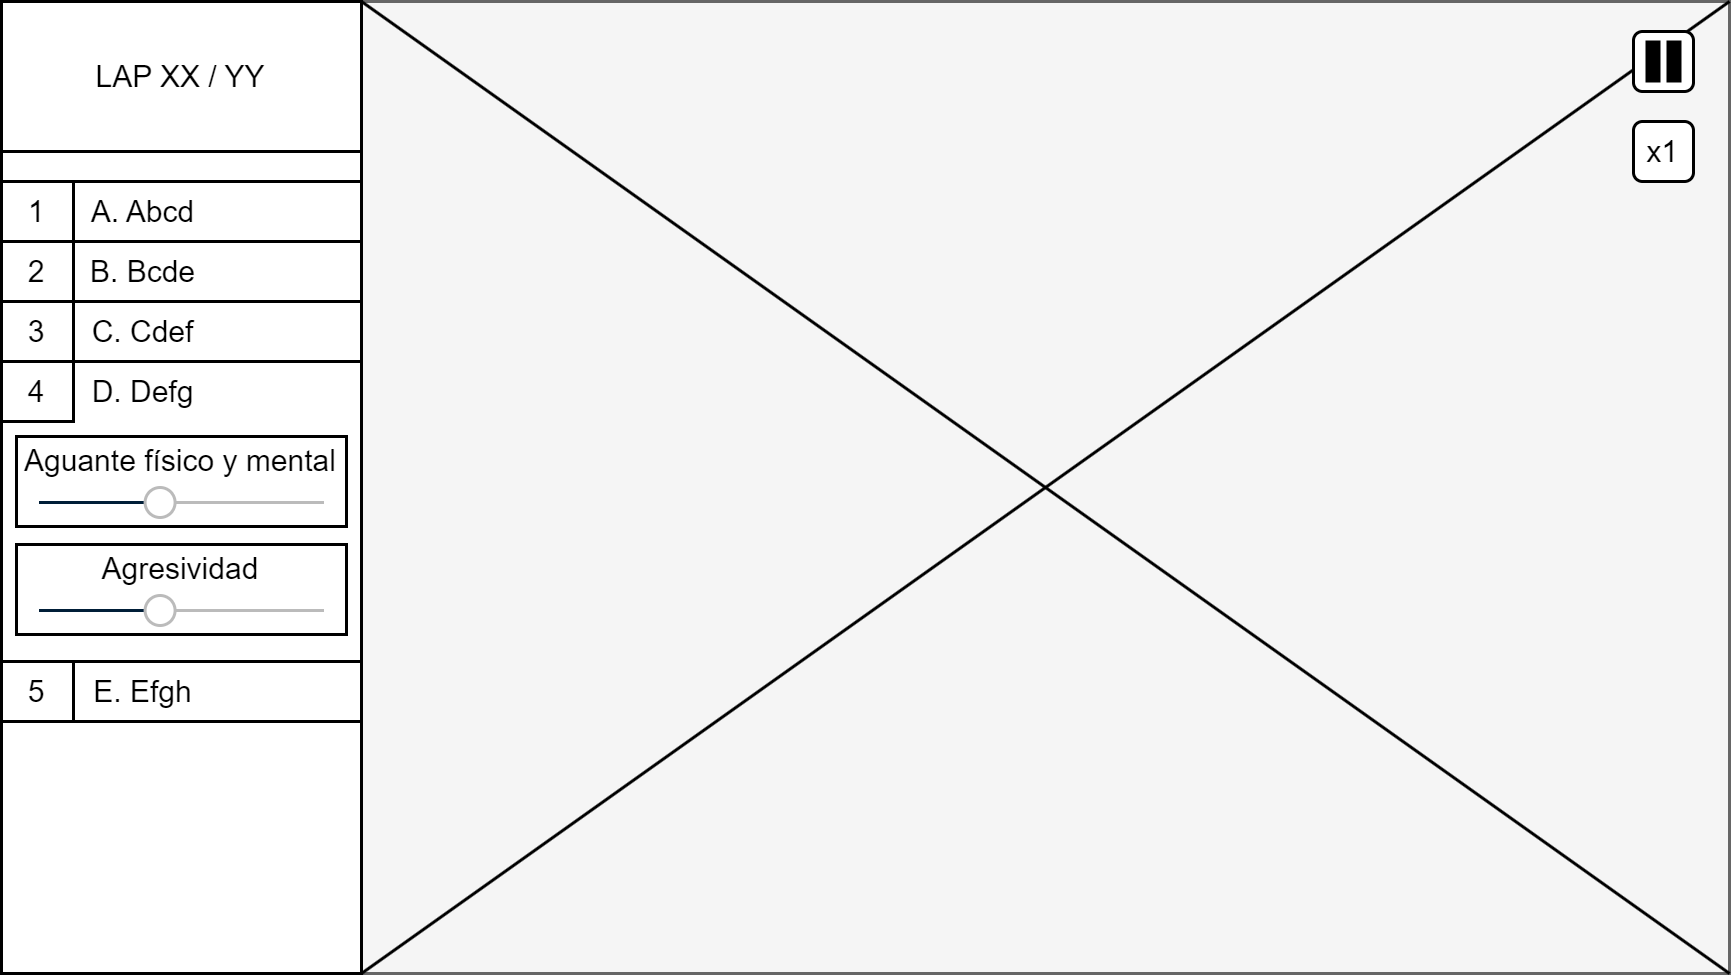
\includegraphics[width=\textwidth]{imagenes/pag2.png}
    \caption{Interfaz de las opciones durante la carrera.}
\end{figure}

\section{Diagrama de navegación}

La navegación por la interfaz de usuario en la aplicación es relativamente sencilla, al estar formada por dos pantallas: el configurador de simulación y la carrera en curso.

\bigskip
\newpage
El diagrama de navegación de la aplicación se encuentra a continuación:

% foto del diagrama de navegacion
\begin{figure}[H]
    \centering
    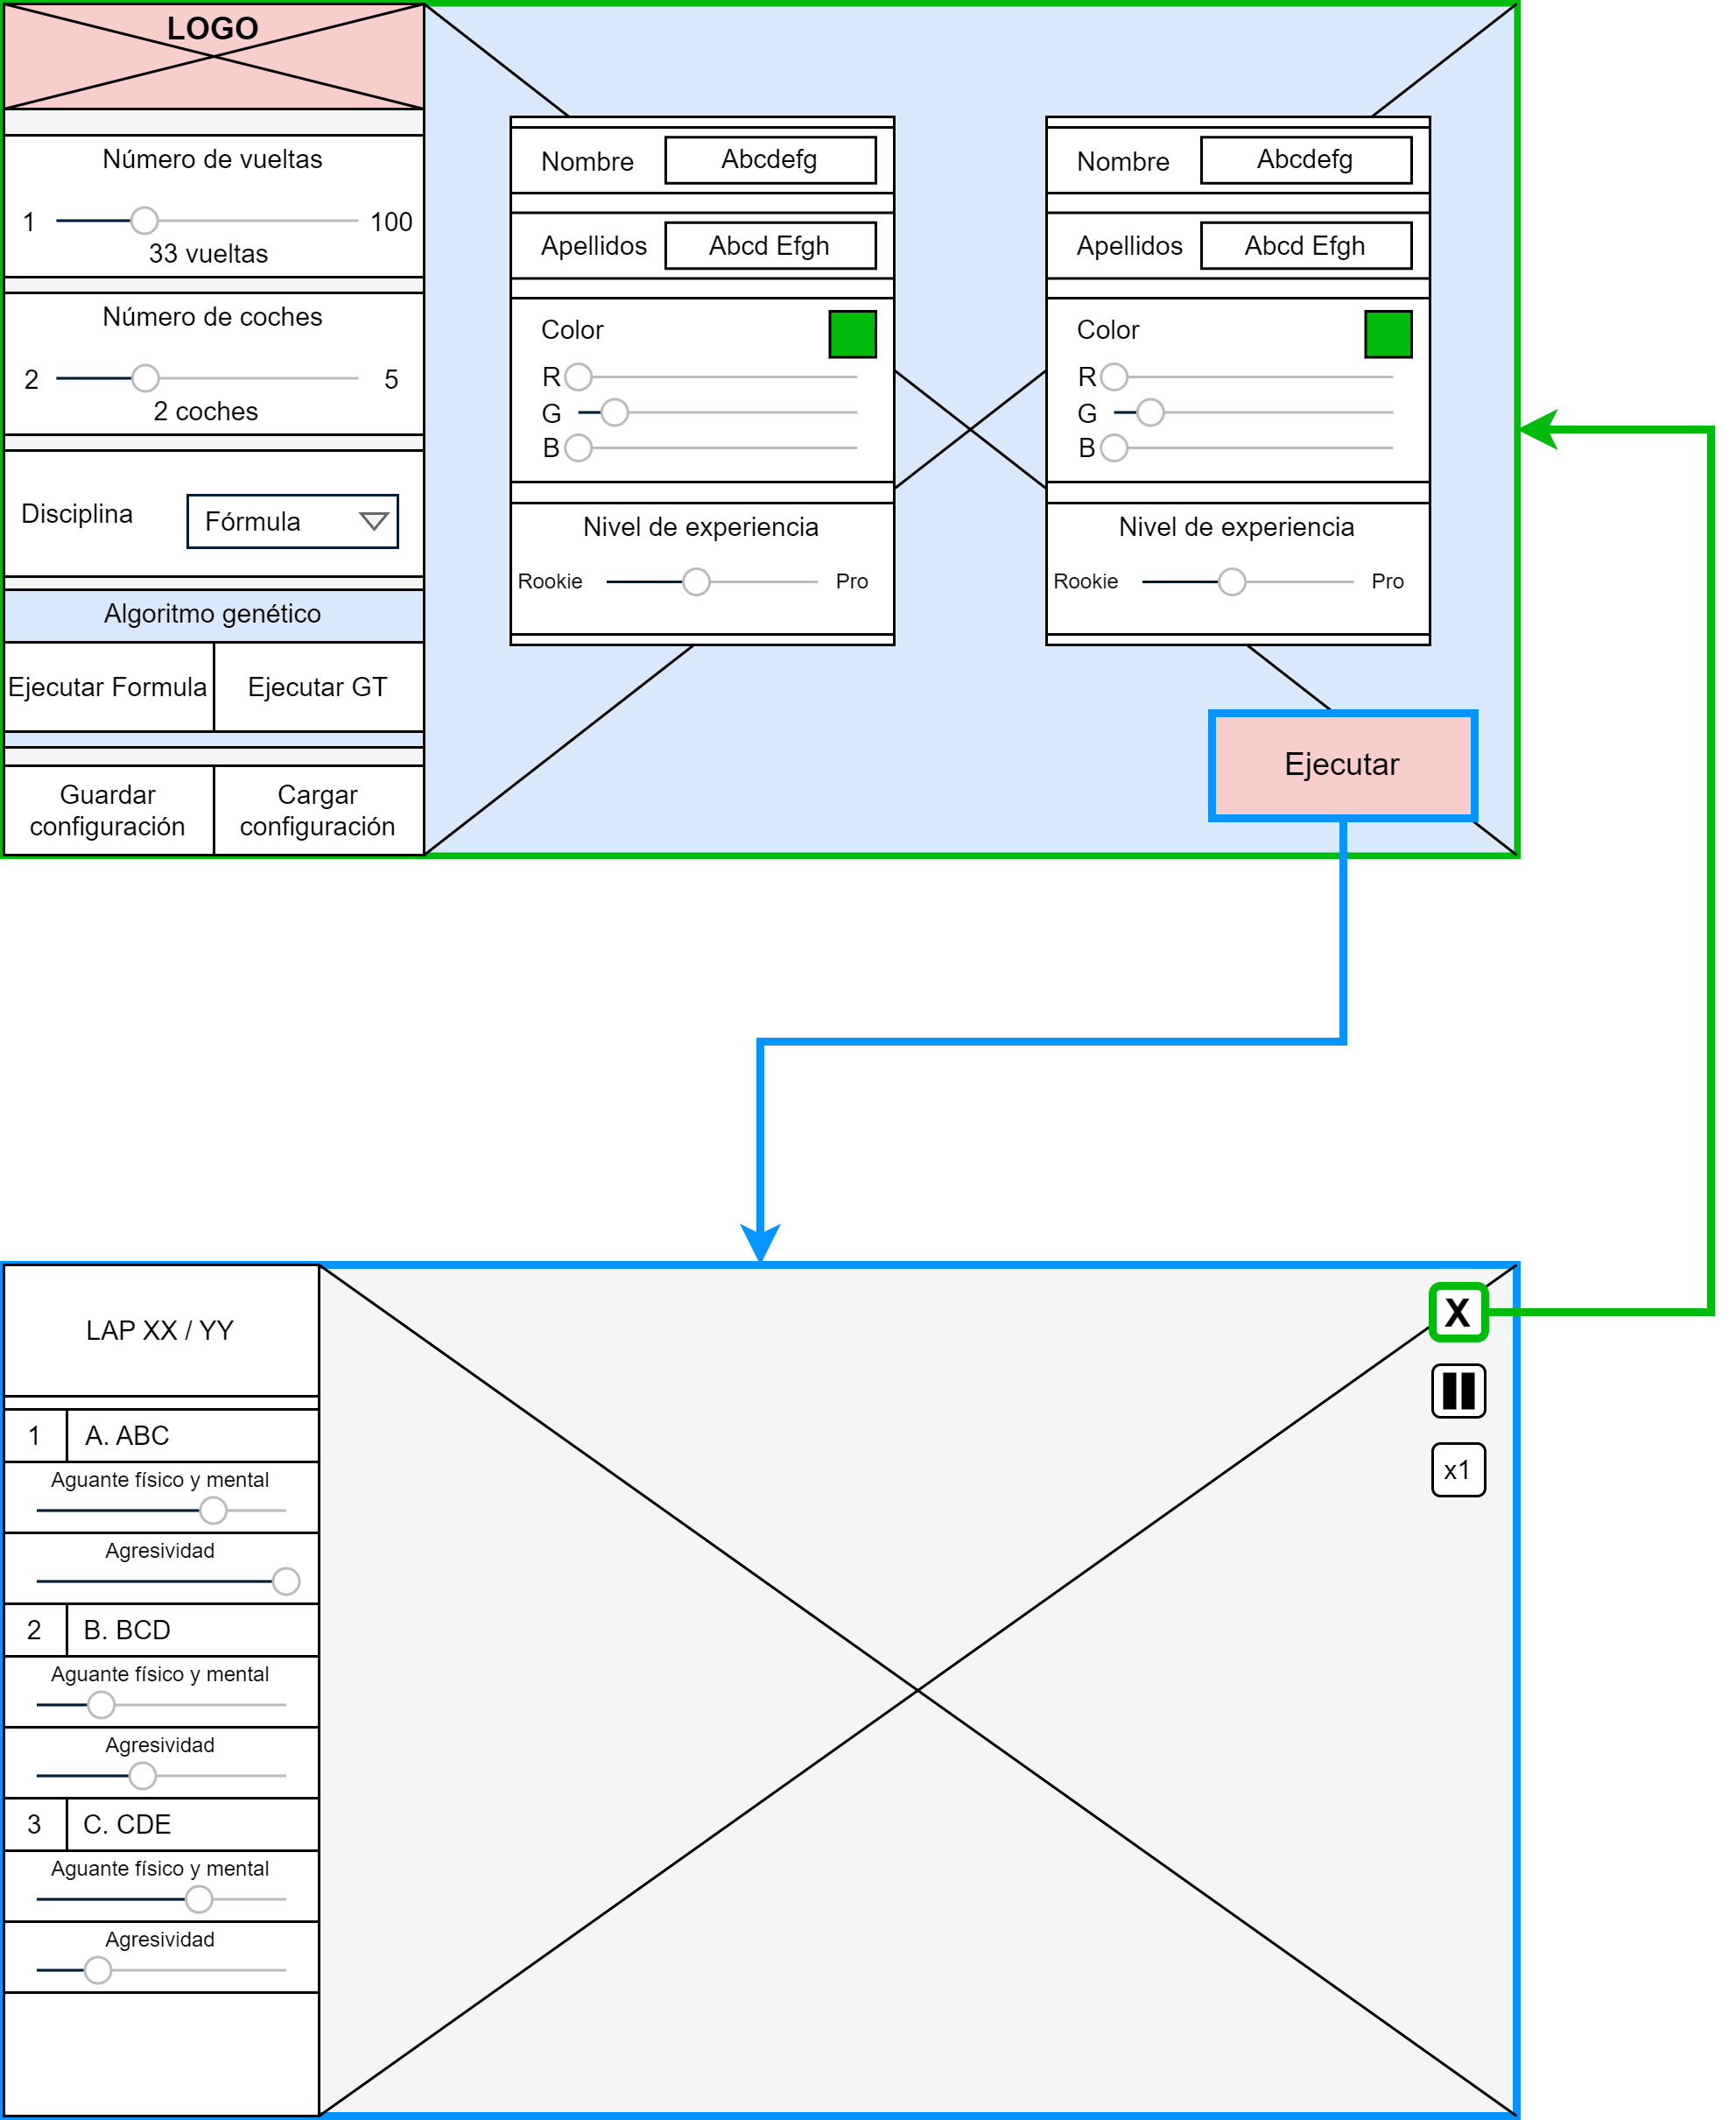
\includegraphics[width=0.9\textwidth]{imagenes/nav.png}
    \caption{Diagrama de navegación de la interfaz de usuario de la aplicación.}
 \end{figure}

 Como se puede observar, la navegación por la aplicación es sencilla, al solo tener dos pantallas y un solo botón para ir a la siguiente. Si se pulsa sobre el botón de ejecutar en el configurador de la carrera, se procederá a cargar la simulación y dará comienzo la carrera.